\chapter{Methods} 
\label{ch:methods:methods}
Time perception is convoluted with motor functions.
As discussed in the \hyperref[ch:intro:intro]{first chapter}, disentangling the two has proven to be difficult, and sometimes, overlooked.
Using original behavioral tasks, designed with the above concern in mind, might shed new light on this matter.
In this chapter, I present a novel behavioral paradigm that allowed monitoring the locomotive activity of the animals as well as their timing performance.
I also provide technical details about different variants of this paradigm used in this work.
I also present all the experimental and analytical methods used in this project.

\section{Experimental Tools} \label{ch:methods:exp}
In this section, all the conditions used in the time-estimation experiments and other experimental methods are described.

\subsection{Subjects}
Subjects were male Long-Evans rats.
They were 12 weeks old at the beginning of the experiments, housed in groups of 4 rats in temperature-controlled ventilated racks and kept under 12~h--12~h light/dark cycle.
All the experiments were performed during the light cycle.
Food was available \textit{ad libitum} in their homecage.
Rats had access to water for 30~min after every experimental session, while their body weights were regularly measured.
No animal was excluded from further analysis.
All experimental procedures were conducted in accordance with standard ethical guidelines (European Communities Directive 86/60 - EEC) and were approved by the relevant national ethics committee (Minist\`{e}re de l'enseignement sup\'{e}rieur et de la recherche, France).

\subsection{Task Apparatus}
Four identical treadmills were used for the experiments.
Each treadmill was placed inside a ventilated sound-attenuating box (\Autoref{fig:methods:taskRules}{a}).
Treadmills were 90~cm long and 14~cm wide, surrounded by plexiglass walls such that the animals were completely confined on top of the treadmill belt.
Treadmill belt covered the entire floor surface and was driven by a brushless digital motor (BGB 44 SI, Dunkermotoren).
A reward delivery port (solenoid valve) was installed on the front (relative to the turning direction of the belt) wall of the treadmill and released a $\sim$80~$\mu$L drop of 10\% sucrose water solution in case of a full reward.
An infrared beam was placed 10~cm from the reward port.
The first interruption of the beam was registered as \gls{et}.
A loudspeaker, placed outside the treadmill, was used to play an auditory noise (1.5~kHz, 65~db) to signal error trials.
Two strips of LED lights were mounted on the ceiling along the treadmill to provide visible and infrared lighting during trials and intertrials, respectively.
The animals' position was tracked via an overhead camera (Basler scout, 25~fps).
A custom-made algorithm detected the white coating of the rats and recorded its centroid as animals' position.
The entire setup was fully automated by a custom-made program (LabVIEW, National Instruments).
Experimenter was never present in the behavioral laboratory during the experiments.
\begin{SCfigure}%[bt!]
    \includegraphics[scale=1]{ch-methods/figures/TaskRulesFULL.pdf}
    \caption[Treadmill Task]
        {\textbf{Treadmill task and trial types.}
        \textbf{a)}
        Rats were enclosed on a powered treadmill.
        The infrared beam marked the reward area (red shaded area).
        During each trial, the belt pushed the animals away from the reward area and the first infrared beam interruption defined the \gls{et}.
        During trials and intertrials, the animal's position was tracked via a ceiling-mounted video camera.
        \textbf{b)}
        Schematic description of a rewarded correct trial.
            \textit{Inset}: the magnitude of the delivered reward dropped linearly as \gls{et} increased (maximum reward at \acrlong{gt}).
            In early stages of training, smaller rewards were delivered for trials with $ET<7$~s.
            However, the smallest \gls{et} value that triggered reward delivery was progressively raised during learning.
        \textbf{c)}
        Schematic description of an error trial.
        Early \glspl{et} triggered an extra-running penalty and an audio noise.
            \textit{Inset}: the duration of the penalty period was 10~s for the shortest \glspl{et} and fell linearly to 1~s for \glspl{et} approaching 7~s.
        \textbf{d)}
        Schematic description of an omission trial (no beam crossing between 1.5~s and 15~s).
        \textbf{b-d)}
        Note that \glspl{et} started to be detected 1.5~s after the motor start.
    }
    \label{fig:methods:taskRules}
\end{SCfigure}

\subsection{Habituation} \label{ch:methods:habituation}
Animals were handled 30~min per day for 3 days, then habituated to the treadmill for 3 to 5 daily sessions of 30~min, while the treadmill's motor remained turned off and a drop of reward was delivered every minute.
Habituation sessions resulted in systematic consumption of the reward upon delivery.

\subsection{Treadmill Task} \label{ch:methods:normalTrdTask}
Training started after handling and habituation sessions.
Each animal was trained once a day, 5 times a week (no training on weekends).
Each of the daily sessions lasted for 55~min and contained $\sim$130 trials.
Each trial started by turning the treadmill motor on at a fixed speed of 10~cm/s. 
One second before motor onset, the ambient light was turned on (to warn the animals of the imminence of the belt movement). 
The conveyor belt moved toward the rear of the treadmill (\Autoref{fig:methods:taskRules}{a}). 
Three types of trials were defined based on the time the animal first interrupted the infrared beam, i.e., the \gls{et}, relative to the \gls{gt}.
Trials in which animals entered the reward area after the \gls{gt} were classified as \emph{correct} ($7\leq ET<15$, \Autoref{fig:methods:taskRules}{b}).
Trials in which animals entered the reward area before the \gls{gt} were classified as \emph{error} ($1.5\leq ET<7$, \Autoref{fig:methods:taskRules}{c}).
In case no infrared beam interruptions were registered in 15~s, the trial ended and was classified as \emph{omission} (\Autoref{fig:methods:taskRules}{d}).
The infrared beam was inactive during the first 1.5~s ($ET<1.5$) to give the opportunity to the animals to leave (passively or actively) the reward area at the beginning of each trial.
Additionally, the exact value of the \gls{et} determined a reward/punishment ratio.
The reward was a drop of sucrose solution and the punishment was a period of extra running.
The running penalty started when the animals erroneously crossed the infrared detector before \gls{gt} (error trial) and its duration varied between 10~s and 1~s, according to the error magnitude (\Autoref{fig:methods:taskRules}{c, inset}).
Thus, to maximize reward collection and minimize running time, animals should cross the infrared beam just after the \gls{gt}.

\subsubsection{Reward Profile} \label{ch:methods:reward}
The magnitude of the reward was a function of the \gls{et} and animal's performance in previous sessions.
Reward was maximal at $ET=GT$ and dropped linearly to a minimum (i.e., $\sim 38\%$ of the maximum) for \glspl{et} approaching 15~s (maximum trial duration).
Moreover, in the beginning of the training, partial reward was also delivered for error trials with $ET>ET_0$, where $ET_0$ denotes the minimum threshold for getting a reward.
The magnitude of this additional reward increased linearly from zero for $ET=ET_0$, to its maximum volume for $ET=GT$.
In the first session of training, $ET_0=1.5$~s and for every following session, it was updated to the maximum value of median \glspl{et} of the past sessions.
Once $ET_0$ reached the \gls{gt}, it was not updated anymore (late training reward profile in \Autoref{fig:methods:taskRules}{b, inset}).

\subsection{Alternative Task Conditions}
In addition to the ``normal'' treadmill task described above, several modified versions of the task were also designed to investigate the embodiment hypothesis.
In each of these conditions, a specific parameter of the task was altered, allowing us to study its effect on animals' performance.

\subsubsection{Variable Speed Condition}
In this condition, for each trial, treadmill speed was pseudo-randomly drawn from a uniform distribution between 5 and 30~cm/s.
During any given trial, the speed remained constant.
We used 5~cm/s as the lowest treadmill speed, because lower speeds generated choppy movements of the conveyor belt.
Also, velocities higher than 30~cm/s were not used, to avoid any physical harm to the animals.

\subsubsection{No-timeout Condition}
In the control condition, the infrared beam was not active during the first 1.5~s of the trials. 
This \emph{timeout} period was sufficient to let the animals be carried out of the reward area by the treadmill, provided they did not move forward.
In the ``no-timeout'' condition, the infrared beam was activated as soon as the trial started.
Thus, in this condition, error trials corresponded to \glspl{et} between 0 and 7~s.
Consequently, animals were penalized if they were in the reward area when the trial started (i.e., $ET=0$~s).

\subsubsection{Short Goal Time Condition}
In this condition, the \gls{gt} was set to 3.5~s, half the value for the control condition.
The reward profile in this condition followed the same rules as for the control condition, except that reward was maximal at $ET=GT=3.5$~s.
Two different groups of animals were trained in this condition, one with treadmill speed set to the normal value of 10~cm/s, and another with treadmill running twice as fast.
In the short goal time condition, we also examined if the increased variability in \gls{et} could be attenuated when the penalty associated with early \gls{et} was increased and when reward magnitude was decreased for late \glspl{et}.
This was implemented by doubling the treadmill speed during the penalty period (from 10~cm/s to 20~cm/s), and the reward was delivered for a narrower window of \glspl{et} (maximal reward at $ET=GT=3.5$~s, and no reward after $ET=4.5$~s).
For proper comparison, we also examined the behavior of rats trained with $GT=7$~s when the running penalty was increased and the reward was decreased for late \glspl{et} (maximal reward at $ET=GT=7$~s, and no reward after $ET=9$~s).

\subsubsection{Immobile Condition}
In this condition, the treadmill motor was never turned on.
The ambient light was turned on during the trials and turned off during the intertrials.
Error trials were penalized by an audio noise and extended exposure to the ambient light.

\subsection{Reverse Treadmill Task} \label{ch:methods:rev}


\subsection{Locomotion Task} \label{ch:methods:loco}
\section{Technical Tools} \label{ch:methods:tech}
In this section, I specify the details of the techniques used in experiments and data processing.
\subsection{Striatal Lesion} \label{ch:method:lesion}
\begin{figure}[bth!]
 \begin{center}
	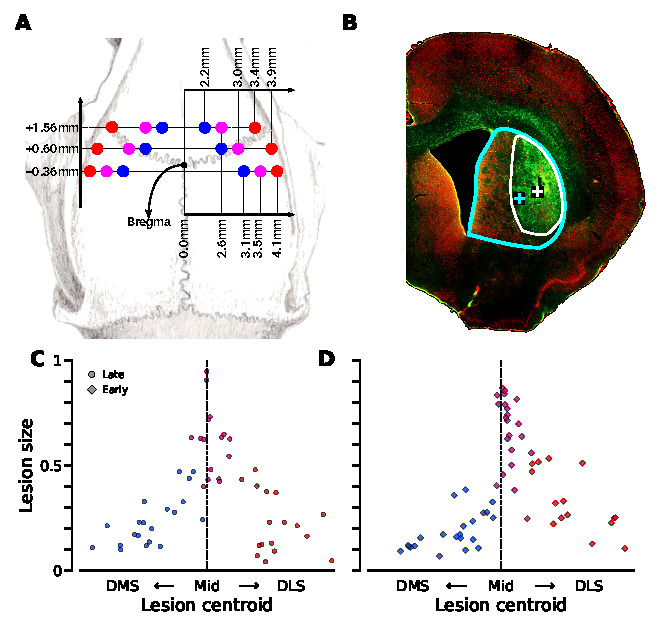
\includegraphics[width=0.9\linewidth]{ch-methods/figures/LesionSizeLocation.pdf}
	\caption[]
	{\textbf{dS Lesion quantification.}
	\textbf{(A)} Schematic of the lesion sites.
	\textbf{(B)} Illustration of the quantification of the lesion size. For each coronal slide and hemi-striatum, the contour of the lesion was manually outlined using GFAP staining.
	The relative size of the lesion (compared to the full dS, manually outlined on the NeuN staining) and the coordinates of the lesion/striatum centroid was calculated.
	For each animal, the size and laterality was obtained by averaging data along the anteroposterior axis, for both left and right hemispheres.
	\textbf{(C,D)} Lesion size versus laterality for animals that underwent lesion before (Early) and after (Late) extensive practice.
	Lesion quantification was performed blindly relative to behavioral analysis.
	}
	\label{fig:method:LesionSizeLocation}
 \end{center}
\end{figure}
Anesthesia was induced with an intraperitoneal (IP) injection of a mixture of 100~mg/kg ketamine and 10~mg/kg xylazine and was maintained during the surgery with inhalant isoflurane gas (less than 3\%).
After shaving and cleaning the scalp, the animal was placed in the stereotaxic frame (Kopf instruments) and a local analgesic (lidocaine) was injected under the scalp.
Then, an incision along the midline of the skull was made, followed by cleaning the exposed skull and drilling the craniotomies above the targeted areas.
To perform fiber-sparing lesion of the \gls{ds}, ibotenic acid (1\% in 0.1~M~NaOH, Fisher Scientific) was infused (Pump 11 Elite Nanomite, Harvard Apparatus, using a 10~$\mu$L WPI Nanofil syringe) in 6 specular sites bilaterally, at a rate of 90~nL/min.
The needle remained in-place for 10~min following the injection to allow for the diffusion of the excitotoxic drug.
Then, the needle was retracted slowly to avoid backflow of the drug.
Once all the injections were performed, craniotomies were filled with bone wax, the skull was disinfected, and the skin was sutured.
Animals were allowed to recover for two weeks before resuming behavioral training.
After surgery, animals were housed alone for 3 days, to avoid getting hurt by the cagemates, and were force-fed if needed.
Injection coordinates (in~mm, with reference to Bregma, according to Paxinos) are shown in \Autoref{fig:method:LesionSizeLocation}{A} (each injection at $-5.6$~mm dorsoventral).
The infused volume in each site was 200~nL for DLS and DMS lesions, and 400~nL for \gls{ds} lesions.

\subsection{Immunohistochemistry}
At the end of the experiments, animals were euthanized with an overdose IP injection of $\sim$2~mL pentobarbital.
Then, they were perfused with 4\% paraformaldehyde and their brains were harvested for histological analysis of the lesion size and location.
Brains were coronally sliced on a vibratome at 60~$\mu$m thickness.
For each animal, six sections spanning the \gls{ds} along the rostrocaudal axis were selected (usually the following slice numbers: 5, 15, 25, 35, 45, and 55 for consistency) and submerged in 0.1~M~PBS.
Then, PBS was replaced with citrate buffer (10~mM) for 10~min at room temperature.
Next, slices were submerged in a blocking solution, consisting of PBS with 0.3\% triton and 15\% normal goat serum for 120~min at room temperature.
Then, the solution was replaced with another consisting of 2~$\mu$L mouse anti-NeuN antibody (Merks Millipore, MAB377) and 0.5~$\mu$L of rabbit anti-GFAP antibody (Agilent, Z033429-2) diluted in 200~$\mu$L of the blocking solution, kept overnight at 4~\textcelsius.
Sections were then rinsed twice in PBS, 10~min each, at room temperature, before being submerged again in 1~$\mu$L of donkey anti-mouse antibody (Al555, red), 1~$\mu$L of donkey anti-rabbit antibody (Al488, green) diluted in 400~$\mu$L of PBS for 120~min at room temperature.
Finally, they were washed twice in PBS, for 10~min each time, and mounted for microscopy.

\subsection{Lesion Quantification}
Whole slices were imaged using an Apotome microscope (Zeiss, 28126), and stitched together in the processing software (Zeiss Zen).
Then for each slice, the ventricule, the striatum, and the lesioned area were manually outlined (\Autoref{fig:method:LesionSizeLocation}{B}) bilaterally in the image processing software (ImageJ, Fiji).
The size and the centroid coordinates were automatically computed for all of the above-mentioned areas.
Next, the anteroposterior location of each slice was also approximated according to the rat brain atlas (Paxinos).
\par
The lesion size reported in this paper is the ratio of the lesion volume over the volume of the striatum.
Both regions of interest (lesion and striatum) were approximated as a truncated cone between any two consecutive sections, and the volume was accordingly calculated and summed up.
\Autoref{fig:method:LesionSizeLocation}{C-D} show the lesion coordinates of all the animals trained in the normal treadmill task.
The type of the lesion (\gls{dls}, \gls{dms} or \gls{ds}) was determined visually and confirmed by comparing the centroid location of the lesion to that of the entire striatum.
Animals with a \gls{dls} lesion in one hemisphere and a \gls{dms} in another ($n=7$) were excluded from this manuscript.
Four rat brains were imaged improperly, they are automatically removed from any analysis that required the lesion size.


\subsection{Statistics}
All statistical comparisons were performed using resampling methods (permutation test and bootstrapping).
These non-parametric methods alleviate many concerns in traditional statistical hypothesis tests, such as distribution assumptions (e.g., normality assumption under analysis of variance), error inflation due to multiple comparisons, and sensitivity to unbalanced group size.
\par
We used the permutation test to compare the performance of two groups of animals during training on a session-by-session basis, such as in \Autoref{fig:time:varTrd}{b}, and \Autoref{fig:lesion:EarlyLesionLearning}{A}.
To simplify the description~\cite[see][for the complete description]{Fujisawa2008NN}, let's assume, as in \Autoref{fig:time:varTrd}{b}, we have ${\mathbf{X}=[X_1, X_2,...,X_n]}$, where $X_i$ is the set of \glspl{et} of all the animals in session~$i$.
Similarly, we have $\mathbf{Y}$ that contains \glspl{et} from another experimental condition.
Here, the null hypothesis states that the assignment of each data point in $X_i$ and $Y_i$ to either $\mathbf{X}$ or $\mathbf{Y}$ is random, hence there is no difference between $\mathbf{X}$ and $\mathbf{Y}$.
\par
In short, the test statistic was defined as the difference between smoothed (using Gaussian kernel with $\sigma =0.05$) average of $\mathbf{X}$ and $\mathbf{Y}$ for each session~$i$: $D_0(i)$.
I then generated one set of surrogate data by assigning \gls{et} of each animal in session $i$ to either $X_i$ or $Y_i$, randomly.
For each set of surrogate data, the test statistic was similarly calculated, i.e.,~$D_m(i)$.
This process was repeated 10,000 times for all the statistical comparisons in this manuscript, obtaining: $D_1(i),\ldots,D_{10000}(i)$.
\par
At this step, two-tailed pointwise p-values could be directly calculated for each $i$, from the $D_m(i)$ quantiles~\cite{Fujisawa2008NN}.
Moreover, to compensate for the issue of multiple comparisons, we defined global bands of significant differences along the session index dimension.
From 10,000 sets of surrogate data, a band of the largest $\alpha$-percentile was constructed, such that less than 5\% of $D_m(i)$s broke the band at any given session $i$.
This band (denoted as the \textit{global band}) represents the threshold for significance, and any break-point by $D_0(i)$ at any $i$ is a point of significant difference between $\mathbf{X}$ and $\mathbf{Y}$.
\par
A similar permutation test was also used when comparing only two sets of \textit{unpaired} data points (such as in \Autoref{fig:time:shortSharp}{e}, comparing control vs.\ short~GT groups).
The same algorithm was employed, having only one value for index $i$.
If none of the $D_m(i)$s exceeded $D_0(i)$, the value $p<0.0001$ was reported (i.e., less than one chance in 10,000).
\par
For paired comparisons (such as in \Autoref{fig:time:varTrd}{f} and in \Autoref{fig:lesion:rev}{C}), I generated the bootstrap distribution of mean differences ($n=10000$ with replacement).
Significance was reported if 95\% confidence interval (CI) of the pairwise differences differed from zero (i.e., zero was not within the CI)~\cite{Efron1994}.
For example, in \Autoref{fig:time:varTrd}{f, right}, the 95\% CI of pairwise differences is $(19, 27)$.
Since this interval does not contain zero, it is reported significant, whereas in \Autoref{fig:time:shortSharp}{e}, the CI of the comparison between normal and sharp short~GT is $(-0.17, +0.01)$ which includes zero, and hence is reported non-significant.
\par
Exceptionally, for the comparison in \Autoref{fig:time:shortSharp}{h}, even though it is not paired, I used bootstrapping, because I did not have enough data points to perform the permutation test.
In this case, the resampled distribution ($n=10000$ with replacement) for each group was calculated, and it was reported significant, since the distributions did not overlap at 95\% CI.
\par
Finally, in \Autoref{fig:time:ImmTrd}{f}, I used repeated measures correlation implemented in the Pingouin package~\cite{PingouinToolbox}.
This technique relaxes the assumption of independent data points, since each animal contributes more than one to the analysis.
\section{Data Analysis} 
\label{ch:methods:dataAnalysis}

Data from each behavioral session was stored in separate text files, containing position information, entrance times, treadmill speeds, and all the task parameters.
Position information was then smoothed (Gaussian kernel, $\sigma = 0.3$~s).
The entire data processing pipeline was implemented in python, using open-source libraries and custom-made scripts.
We used a series of Jupyter Notebooks to process, quantify, and visualize every aspect of behavior, to develop and run the reinforcement learning algorithms, and to generate all the figures in this manuscript.
All the Jupyter Notebooks, as well as the raw data necessary for full replication of the figures and videos will be publicly available via the Open Science Foundation.

\subsubsection*{Motor Routine Definition}
We quantified the percentage of trials in which animals performed the wait-and-run motor routine in each session (Fig. 1 I).
A trial was considered \textit{routine} if all the following three conditions were met:
1)~the animal started the trial in the front~(initial position $< 30 cm$);
2)~the animal reached the rear portion of the treadmill during the trial~(maximum trial position $>50 cm$);
3)~the animal completed the trial (i.e., it crossed the infrared beam).

\subsubsection*{Speed Calculation}
Unless otherwise stated, speed in this manuscript refers to the velocity with which animals crossed the treadmill toward the reward port.
For every trial, it is calculated based on the time the animal takes to run from 60~cm to 40~cm along the treadmill.
Speed for each training session is the average speed across its trials (Fig. 1~J).
Furthermore, in Fig.~4B, we categorized the animals based on whether they had an effect on their running speed after dS lesion (black), or not (gray).
Animals were assigned to the black group ($\Delta$Speed$<0$) if the average speed of 5 consecutive stable sessions after the lesion (i.e., session $+8$ to $+13$) were lower than that of 5 consecutive sessions before the surgery (i.e., sessions $-5$ to $-1$).


\subsubsection*{Anti Routine Definition}
Percentage of anti routine trials is analogous to the percentage of routine trials, only in the reverse treadmill.
A trial was considered \textit{anti routine} if the following conditions were met:
1)~the animal started the trial in the back (initial position $> 60 cm$);
2)~the animal completed the trial (i.e., it crossed the infrared beam).


\subsubsection*{Definition of Frontal Trials}
Frontal trials are defined as trials in which the animal remained in the frontal portion of the treadmill (i.e., position $<30$~cm) for the first 5~s after trial onset.


\subsubsection*{Speed Modulation Analysis}
In Fig.~3D, we split the trajectories that strictly followed the wait-and-run routine (see the definition of the Max. Pos.) into trials with the maximum position between 40 and 60~cm (Mid) and those between 70 and 90~cm (Back).
The data was pooled from the last 5 sessions before (Fig.~3D, left) and after (Fig.~3D, right) the lesion.
To improve the reliability, animals were discarded if they did not have at least 10 trials in the Mid and 10 trials in the Back condition (trials that strictly followed the wait-and-run routine, their maximum position was within the range, and for which the speed could have been defined).
Fewer number of animals in the left panel was due to the fact that most animals performed the wait-and-run routine by going all the way to the rear portion of the treadmill, thus not enough Mid trials existed.


\subsubsection*{Definition of Max. Pos.}
The maximum position an animal reached along the treadmill before initiating the run epoch toward the reward in the wait-and-run routine was quantified as Max. Pos. in Fig. 4D.
Therefore, Max. Pos. was only calculated for trials that strictly followed a wait-and-run routine, i.e., total immobility followed by continuous running until reaching the infrared beam.
A trial was qualified if the following conditions were met:
1)~the animal started the trial in the front (initial position $< 30 cm$);
2)~the animal moved at least 10~cm backward (maximum position $\geq 40 cm$);
3)~the animal remained still while being pushed backward by the treadmill (movement shorter than 0.1~s and slower than 5~cm/s were ignored to correct for jitter in position detection);
4)~the animal performed an uninterrupted running epoch (staying immobile or moving backward shorter than 0.1~s was ignored to correct for jitter in position detection);
5)~the animal completed the trial (i.e., it crossed the infrared beam).
Notice that compared to the definition of the routine trials, the threshold for maximum position in the second criterion is relaxed (40~cm, compared to 50~cm) to allow detection of trials with a reduced maximum position.
To increase the reliability, any session with fewer than 10 trials for which Max. Pos. could be defined was excluded from further analysis.
The reported value of Max. Pos. for each session is the average value across its trials (Fig. 4D).


\subsubsection*{Normalizing Speed and Max. Pos.}
In Fig. 4B and~D, to normalize each animal’s performance according to its own behavior prior to the lesion, behavioral measures (speed and Max. Pos.) of individual animals during the illustrated sessions were subtracted from the median value of the respective measure during the pre-lesion sessions.
Animals were included only if the behavioral measure could be defined in at least half of the illustrated sessions.
Different $n$ in panel~D compared to~B, and~B compared to the total number of animals (Fig.1H) is due to this criterion.
